\section{Sonic Generations}

\begin{figure}[htbp]
\begin{center}
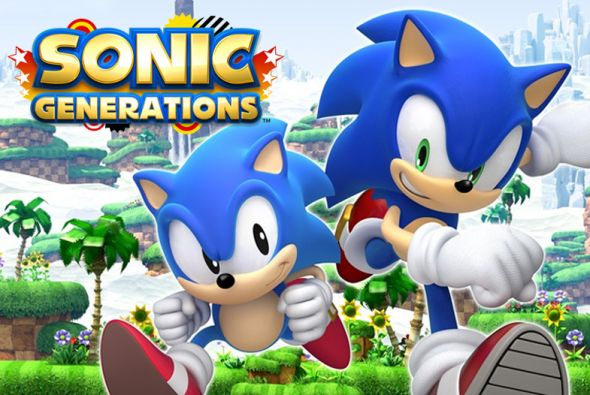
\includegraphics[width=.60\textwidth]{./imagenes/sonic-generations.jpg}
\caption{Sonic Generations}
\label{Sonic Generations}
\end{center}
\end{figure}
Sonic Generations\footnote{\url{http://http://www.sega.com/sonicgenerations/}} es un juego multiplataforma el cual ofrece una nueva experiencia en juego debido a que sus niveles son llevados a escenarios 2D y 3D recreando el ambiente del Sonic antiguo y del Sonic moderno respectivamente. Este juego salió para PS3, Xbox360 y PC el 1 de noviembre del 2011 para celebrar el vigésimo aniversario del nacimiento de Sonic.

Todo empieza cuando los amigos de Sonic estan celebrando su cumpleaños. De repente aparece un enemigo de una hyperdimensión y se los lleva a todos excepto Sonic. Al ocurrir esto, los tiempos chocan y se unen los espacios del Sonic antiguo y del moderno llevando asi todo a una gran confusión. Para poder regresar todo a la normalidad y recuperar a sus amigos, estos erizos deben recorrer los lugares a la velocidad que los identifica y vencer a los mountros que aparezcan en el camino. Al final se enfrentaran con el Dr. Eggman y el Dr. Robotnic siendo estos los enemigos del moderno y antiguo Sonic respectivamente, pero para eliminarlos deberan usar un poder máximo, el cuál solo será otorgado con el uso de las 7 Esmeraldas Caos.

\subsubsection{¿Por qué es uno de mis juegos favoritos?}
\begin{itemize}
\item[Jefferson Rivera] La verdad es que soy un fanático del erizo azul. He jugado todas sus ofertas desde que inicio en la consola Sega con su primer juego Sonic The Hedheog y hasta el momento puedo decir que no me ha decepcionado. Siempre trae nuevas ideas y pues lo que más me gusta es la velocidad que contiene este juego. El erizo avanza tan rápido que siempre debes estar atento a lo que sucede en el desarrollo del mismo. 
\end{itemize}
